\documentclass[a4paper,10pt]{article}
\usepackage[utf8]{inputenc}
\usepackage{amsmath}
\usepackage{graphicx}
\usepackage{hyperref}

%opening
\title{WP 1.1 Mathematical Foundations}
\author{J. G. P. Vermeulen}

\begin{document}

\maketitle

\section{Contents}

This works package details the mathematical foundations for the thesis work. This will be split up into several sections:
\begin{itemize}
\item Coordinate systems and transformations
\item Three-body orbital mechanics (summary)
\item Definitions for the numerical methods
\item Definitions for the Kalman filter methods
\item Definitions for the neural networks
\end{itemize}

\section{Coordinate systems and transformations}
This section will detail the necessary coordinate systems and corresponding transformations.\\

Often, an orbit is expressed in terms of the Keplerian orbital elements:
\begin{itemize}
\item Eccentricity $e$
\item Semi-major axis $a$
\item Inclination $i$
\item Right Ascension of the Ascending Node $\Omega$
\item Argument of Periapsis $\omega$
\item True anomaly at Epoch $\theta$
\end{itemize}

These elements provide a full specification of the orbit in 3D, but they are not that useful for our application. Therefore, some additional coordinate frames are defined, along with transformations. The most important frames are the heliocentric and the geocentric reference frames. Additionally, the camera reference frame of the spacecraft needs to be specified.

\subsection{Heliocentric reference frame}
The heliocentric, or \textit{non-rotating heliocentric ecliptic} reference frame is a non-rotating, quasi-inertial reference frame. As XY-plane, the plane of the ecliptic is used. Therefore, the Z+ direction is perpendicular to the plane of the ecliptic, pointing North. The X+ direction points towards the vernal equinox (first point of Aries). The Y+ direction completes the right-handed coordinate system. The coordinate system is centered on the center of mass of the Sun.

\subsection{Geocentric reference frame}
The geocentric reference frame that will be used is the \textit{non-rotating geocentric ecliptic} reference frame. The geocentric reference frame is defined similar to the heliocentric frame, but centered on the center of mass of the Earth. Note that all axes are parallel: celestial north and the first point of Aries are located at an infinite distance from the origin, and therefore the directions from the Sun and from Earth are parallel.

\subsection{Spacecraft camera reference frame}
To specify the observations of the target in the spacecraft's camera, the spacecraft camera reference frame is defined. In order to specify this coordinate frame, first the spacecraft (quasi-)inertial reference frame is defined. The spacecraft inertial frame is defined similar to the heliocentric and geocentric reference frames, but with the coordinate system centered on the spacecraft center of mass. From this, a simplifying assumption is made: it is assumed the spacecraft focal plane and optical axis coincide with its center of mass. As the dimensions of the spacecraft are negligible compared to the distance to the targets, this assumption is justified. From here, the spacecraft camera reference frame can be defined as the reference frame centered on the intersection of the optical axis of the camera and the camera focal plane, with axis L+ pointing in the direction of the optical axis of the camera (``out'' from the focal plane), M+ pointing to the left and N+ completing the right-handed system by pointing up, both as seen from the focal plane. This is seen in \autoref{fig:cameracoordinates}.

\begin{figure}[htbp]
 \centering
 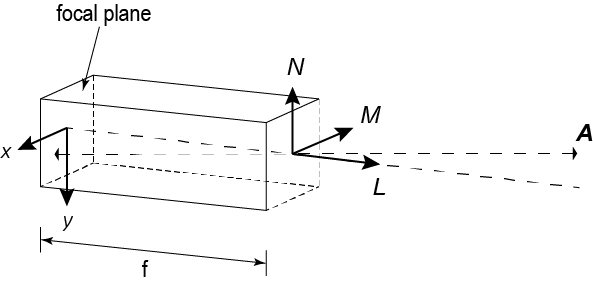
\includegraphics[width=0.6\textwidth]{cameracoordinates.png}
 \caption{Camera reference frame}
 \label{fig:cameracoordinates}
\end{figure}

TRANSFORMATIONS

\section{Alternative coordinate systems}
A problem that will be encountered later in the process is the ``conversion'' from a preliminary orbit determination to an impact threat assessment. For this, it might be necessary to tell the system where Earth is. (alternatively, other metrics such as MOID could be looked at, leading to a system where the target is analysed in more detail from Earth). Instead of giving the system a measure of Earth's location, it might be convenient to define a coordinate system in which both Earth and the Sun (as it is the main gravitational attractor) are fixed. We shall define the Sun-Earth ecliptic reference frame as the right-handed frame with the origin at the center of the Sun, the Z+ axis pointing North perpendicular to the ecliptic, the X+ axis pointing through the center of Earth, and the Y+ axis completing the right-handed system. \\

The advantage of this system is obvious: if we assume Earth's orbit to be circular, the position of Earth will always be $[1, 0, 0]^T~AU$, and therefore the problem simplifies to determining the hazard to that point. However, as the reference frame is no longer non-rotating, the dynamics of the motion vastly complicate.

\section{Transformations}

Most coordinate transformations that are required are quite straightfoward. The transformation between heliocentric frame $h$, geocentric frame $e$ and spacecraft centered frame $s$ can be performed through vector addition. Example for vector $\vec{r}$:
\begin{equation}
 \vec{r}^s = \vec{r}^h - \vec{r_s}^h
\end{equation}
With $\vec{r_s}^h$ denoting the position of the spacecraft in the heliocentric frame. In words: the position of the target in the spacecraft-centered frame is the difference of the position of the target and the position of the spacecraft in any of the other reference frames. \\

Thus, when the position of Sun, Earth and spacecraft are known in each of the respective frames, the coordinate transformation is straightforward. The other coordinate frames require a more elaborate transformation to achieve. The Sun-Earth ecliptic frame $r$ (for rotating) can be achieved by a rotation of the heliocentric frame around the Z-axis. If we define the true anomaly of the Earth $\theta_e$ as 0 at the vernal equinox, we find that:

\begin{equation}
 \vec{r}^r = \mathbf{R_3}(\theta_e) \vec{r}^h
\end{equation}

With $\mathbf{R_3}$ denoting a rotation around the third axis. Similarly, the camera coordinate frame can be achieved by a rotation matrix $\mathbf{C}$ which can be given in terms of twist angle $\phi$, right ascension $\alpha$ and declination $\delta$:
\begin{equation}
 \mathbf{C} = \mathbf{R_3}(\phi)\mathbf{R_1}(90^\circ - \delta)\mathbf{R_3}(\alpha + 90^\circ)
\end{equation}
or:
\begin{equation}
 \mathbf{R_3}(\phi + 90^\circ)\mathbf{R_2}(90^\circ - \delta)\mathbf{R_3}(\alpha)
\end{equation}
Then:
\begin{equation}
 \vec{r}^c = \mathbf{C}(\alpha, \delta, \phi)\vec{r}^s
\end{equation}
The rotation matrices are given by:
\begin{align}
 \mathbf{R_1}(\theta) &= \begin{bmatrix}1 & 0 & 0 \\ 0 & \cos \theta & -\sin \theta \\ 0 & \sin \theta & \cos \theta \end{bmatrix} \\
 \mathbf{R_2}(\theta) &= \begin{bmatrix} \cos \theta & 0 & - \sin \theta \\ 0 & 1 & 0 \\ - \sin \theta & 0 & \cos \theta \end{bmatrix} \\
 \mathbf{R_3}(\theta) &= \begin{bmatrix} \cos \theta & -\sin \theta & 0 \\ \sin \theta & \cos \theta & 0 \\ 0 & 0 & 1 \end{bmatrix}
\end{align}







\section{Two- and Three-body Orbital Mechanics}

The equations of motion need to be known in order to accurately model the asteroids and to e.g. apply the kalman filter and parts of the numerical methods. the equations of motion for two-body problem are simple:

\begin{equation}
 r(\theta) = \frac{a(1-e^2)}{1+e \cos (\theta)}
\end{equation}

As the motion is in a single plane, it is only necessary to know the distance to the barycenter (which can be assumed to coincide with the Sun), and the true anomaly $\theta$. The orbital elements $\Omega$, $i$ and $\omega$ can be seen as Euler angles rotating the coordinate system. If we define the \textit{orbital reference frame} $o$ with X+ towards the periapsis, Z+ perpendicular to the plane of the orbit and Y+ completing the coordinate system right-handed, we can define the following transformations:

\begin{equation}
 \begin{bmatrix}
  x_o \\ y_o \\ z_o
 \end{bmatrix}
 =
 \begin{bmatrix}
  \cos \omega & \sin \omega & 0 \\
  - \sin \omega & \cos \omega & 0 \\
  0 & 0 & 1
 \end{bmatrix}
 \begin{bmatrix}
  1 & 0 & 0 \\
  0 & \cos i & \sin i \\
  0 & -\sin i & \cos i
 \end{bmatrix}
 \begin{bmatrix}
  \cos \Omega & \sin \Omega & 0 \\
  - \sin \Omega & \cos \Omega & 0 \\
  0 & 0 & 1
 \end{bmatrix}
 \begin{bmatrix}
  x_h \\ y_h \\ z_h
 \end{bmatrix}
\end{equation}

Finding the inverse is straightforward: firstly, one should note all matrices are diagonal and thus easily invertible. However, perhaps more intuitively, the rotation sequence can be ``reversed'' by simply reversing the order of the matrices and inverting the sign of the angles (essentially ``rotating'' the system ``back'' into its original orientation):

\begin{equation}
 \begin{bmatrix}
  x_h \\ y_h \\ z_h
 \end{bmatrix}
 =
 \begin{bmatrix}
  \cos -\Omega & \sin -\Omega & 0 \\
  -\sin -\Omega & \cos -\Omega & 0 \\
  0 & 0 & 1
 \end{bmatrix}
 \begin{bmatrix}
  1 & 0 & 0 \\
  0 & \cos -i & \sin -i \\
  0 & -\sin -i & \cos -i
 \end{bmatrix}
 \begin{bmatrix}
  \cos -\omega & \sin -\omega & 0 \\
  - \sin -\omega & \cos -\omega & 0 \\
  0 & 0 & 1
 \end{bmatrix}
 \begin{bmatrix}
  x_o \\ y_o \\ z_o
 \end{bmatrix}
\end{equation}

Lastly, conversion from $r, \theta$ to $x_o, y_o, z_o$ is simple (note that $z_o$ is always zero in the two-body solution as the orbit is planar):
\begin{equation}
 \begin{bmatrix}
  x_o \\ y_o \\ z_o
 \end{bmatrix}
 =
 \begin{bmatrix}
  \cos \theta \\ \sin \theta \\ 0
 \end{bmatrix}
 r
\end{equation}



\section{Numerical Methods}

\section{Kalman Filters}

\section{Artificial Neural Networks}

\end{document}
